%!TEX root = ../thesis.tex
% ******************************* Thesis Appendix B ********************************

\chapter{Histograms of Time To Decision}
%Varying Prior
\begin{landscape}
\centering
\vspace*{\fill}
\section{Histograms of Time To Decision (TTD) with varying Prior Distribution}
\begin{table}[h!]
  \centering
  \begin{tabular}{ | c | c | c | c | c |}
    \hline
    & $\epsilon$-Greedy & Sweep & Random & Saccadic \\
    \hline
    % \multicolumn{2}{c}{Initial Uniform Distribution of Belief Over Grid Cells}\\
    %\hline
    %single RAV
    %\begin{minipage}[c][height][c]{width}
    \rotatebox[origin=c]{90}{Gaussian} & 
    \begin{minipage}[c][49mm][c]{49mm}
      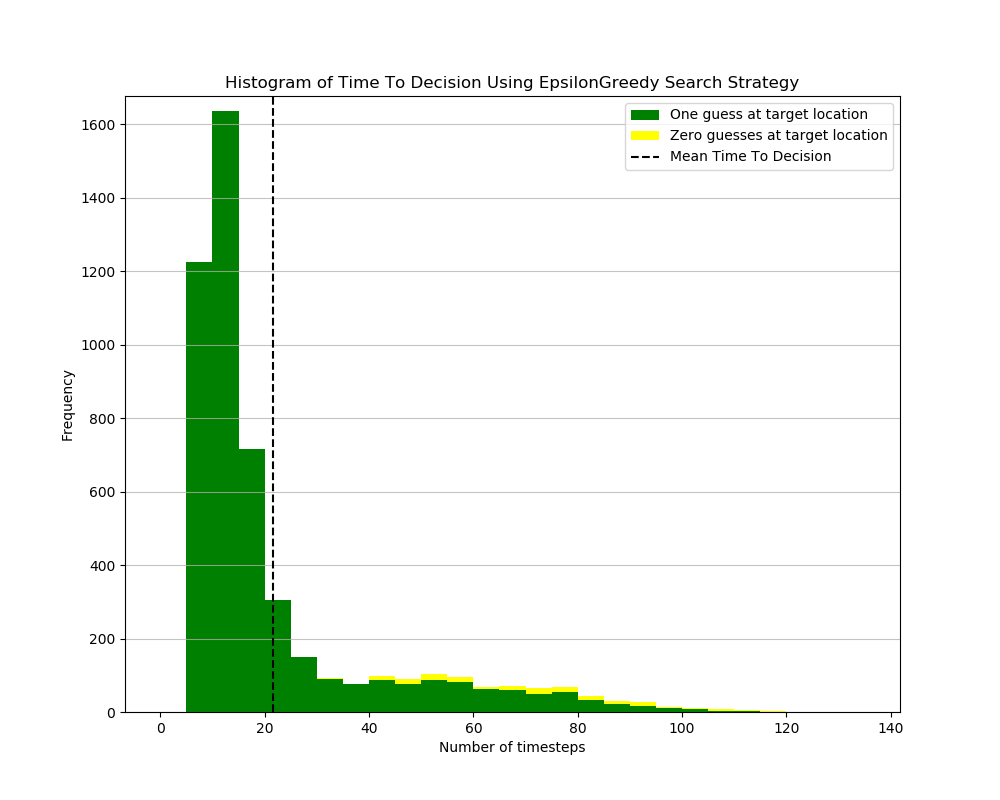
\includegraphics[width=49mm, height=49mm]{Chapters/MultiAgentTargetDetection/Figs/Histograms/VaryingPrior/Gaussian/GaussianEpsilonGreedyHistogram.png}
    \end{minipage}
    &
    %\hline
    %\multicolumn{2}{c}{Initial Discretised Gaussian Distribution of Belief Over Grid Cells (random mean, covariance matrix = [[], []]}\\
    %\hline
    %single RAV
    %\begin{minipage}[c][height][c]{width}
    \begin{minipage}[c][49mm][c]{49mm}
      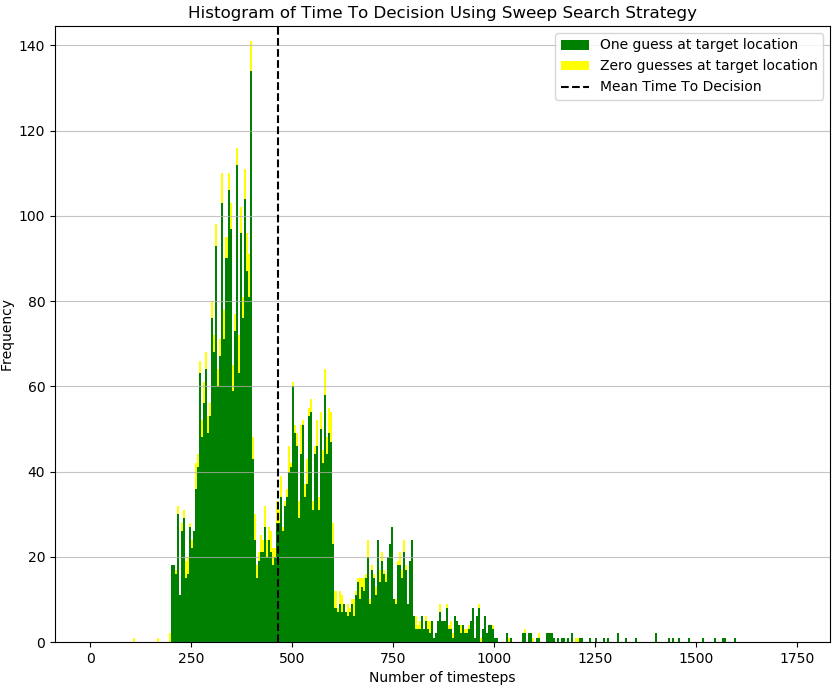
\includegraphics[width=49mm, height=49mm]{Chapters/MultiAgentTargetDetection/Figs/Histograms/VaryingPrior/Gaussian/GaussianSweepHistogram.png}

    \end{minipage}
    &
    \begin{minipage}[c][49mm][c]{49mm}
      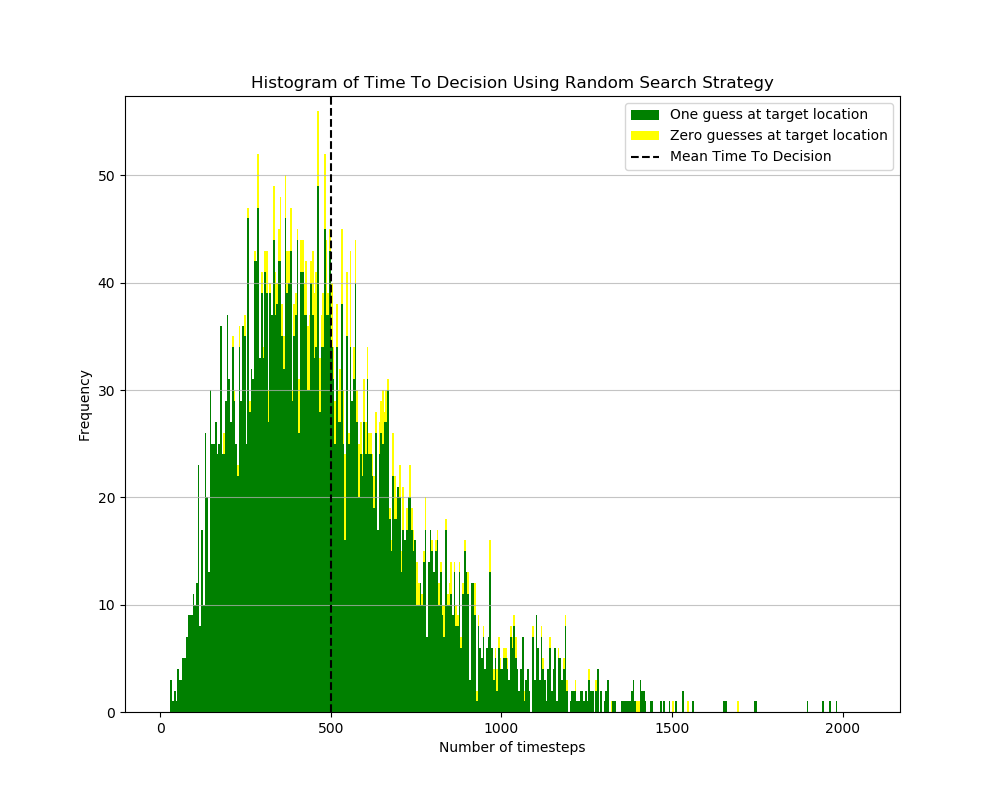
\includegraphics[width=49mm, height=49mm]{Chapters/MultiAgentTargetDetection/Figs/Histograms/VaryingPrior/Gaussian/GaussianRandomHistogram.png}
    \end{minipage}
    &
    \begin{minipage}[c][49mm][c]{49mm}
      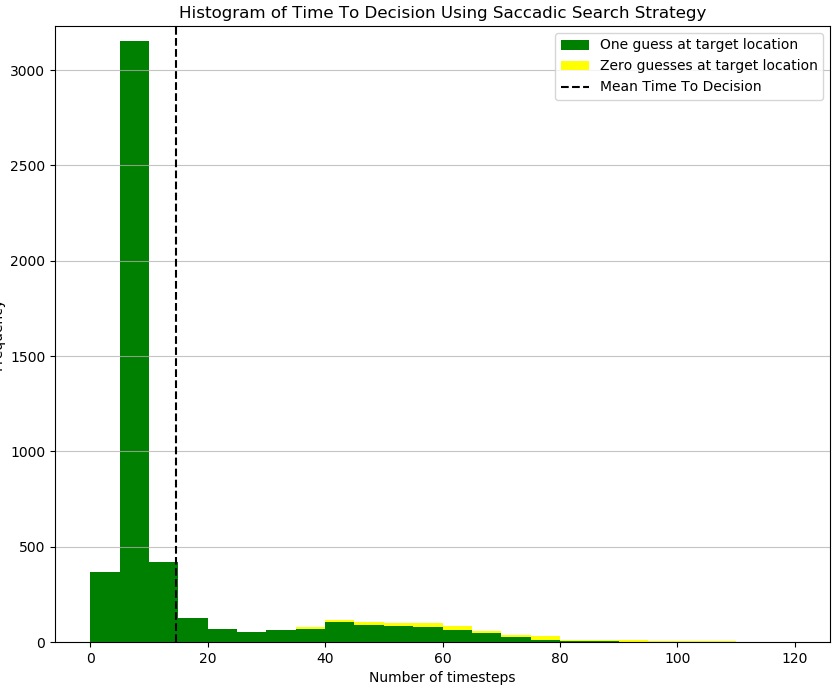
\includegraphics[width=49mm, height=49mm]{Chapters/MultiAgentTargetDetection/Figs/Histograms/VaryingPrior/Gaussian/GaussianSaccadicHistogram.png}
    \end{minipage}
    \\
    %&
    %\small
    %\begin{tabular}{c|c|c|c|c|c|c|c}
    %    Strategy & p(T \Romannum{1}) & p(T \Romannum{2}) & Sim. FPR & Sim. FNR & E[TTD] & Prec. & Rec \\
    %    \hline
    %    $\epsilon$ -Greedy& 4 & 2 & 0.05 & 233.2 & 2303.3 & 2 & 9\\
    %    Sweep & 4 & 2 & 0.05 & 233.2 & 2303.3 & 2 & 9\\
    %    Saccadic & 4 & 2 & 0.05 & 233.2 & 2303.3 & 2 & 9\\
    %    Random & 4 & 2 & 0.05 & 233.2 & 2303.3 & 2 & 9\\

    %\end{tabular}
    %\normalsize
    \rotatebox[origin=c]{90}{Uniform} & 
    \begin{minipage}[c][49mm][c]{49mm}
      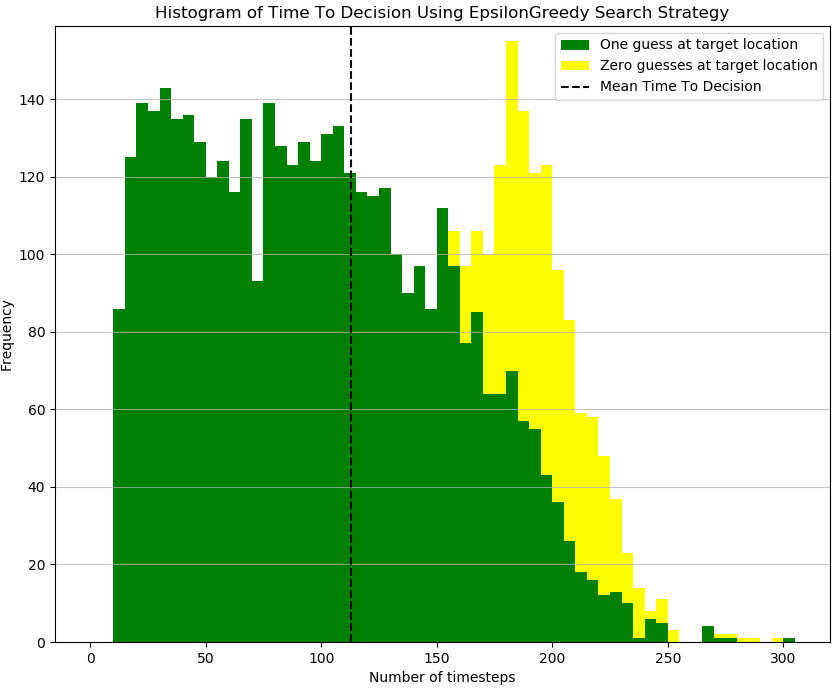
\includegraphics[width=49mm, height=49mm]{Chapters/MultiAgentTargetDetection/Figs/Histograms/VaryingPrior/Uniform/UniformEpsilonGreedyHistogram.png}
    \end{minipage}
    &
    %\hline
    %\multicolumn{2}{c}{Initial Discretised Gaussian Distribution of Belief Over Grid Cells (random mean, covariance matrix = [[], []]}\\
    %\hline
    %single RAV
    %\begin{minipage}[c][height][c]{width}
    \begin{minipage}[c][49mm][c]{49mm}
      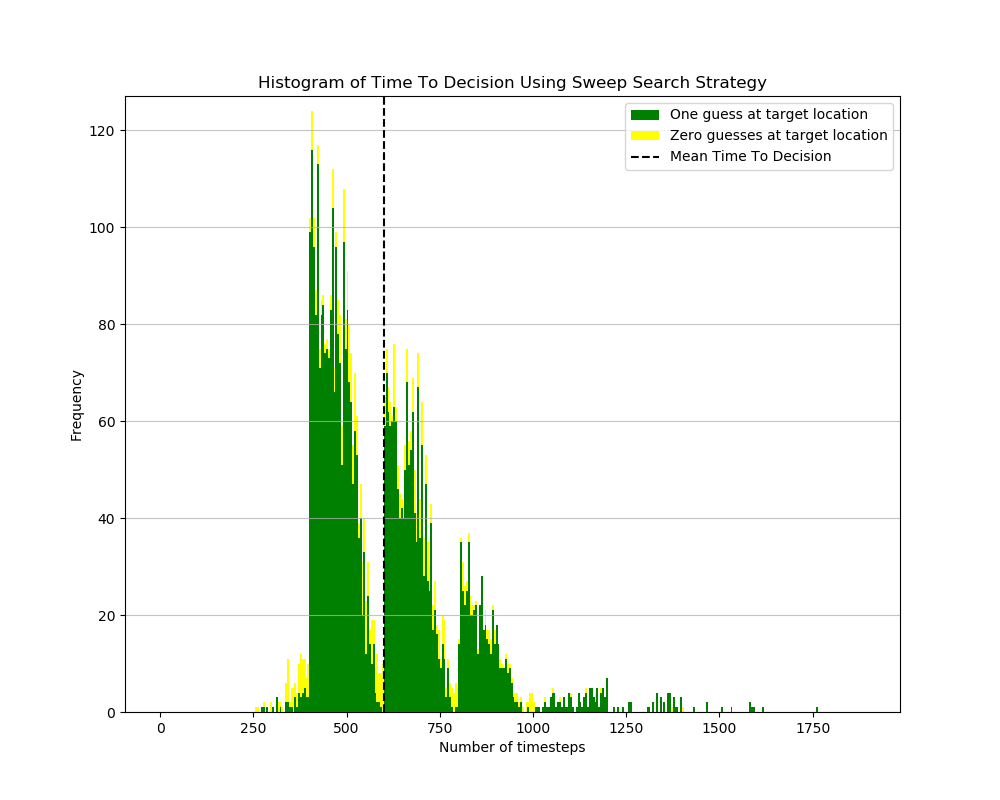
\includegraphics[width=49mm, height=49mm]{Chapters/MultiAgentTargetDetection/Figs/Histograms/VaryingPrior/Uniform/UniformSweepHistogram.png}

    \end{minipage}
    &
    \begin{minipage}[c][49mm][c]{49mm}
      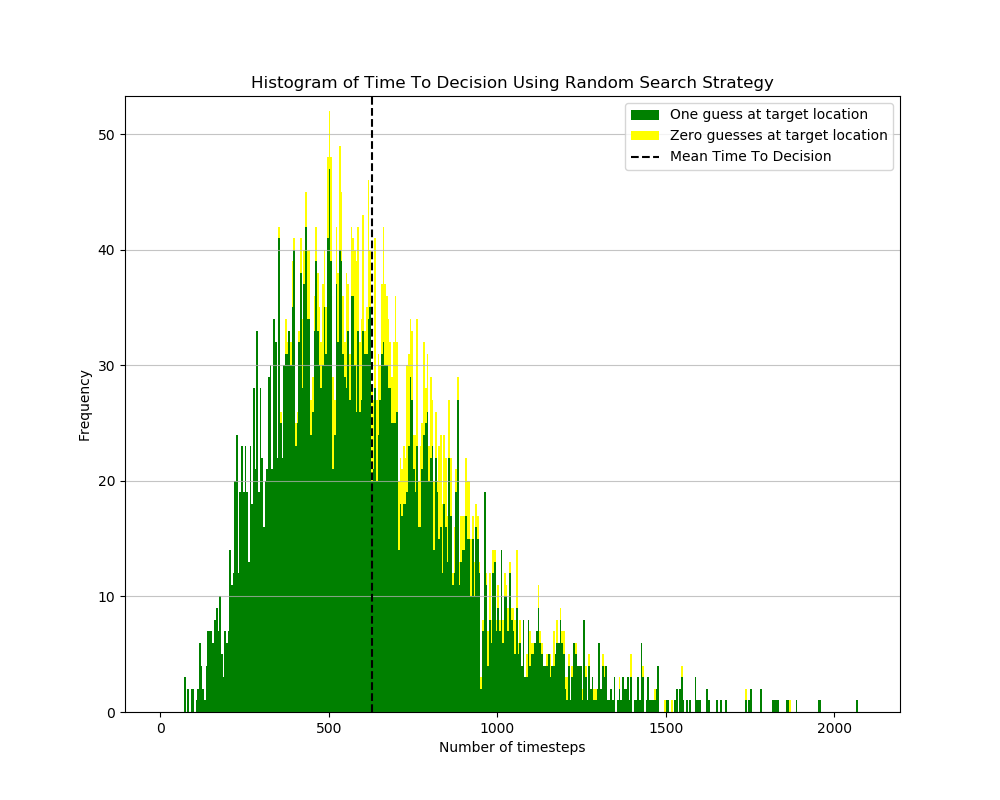
\includegraphics[width=49mm, height=49mm]{Chapters/MultiAgentTargetDetection/Figs/Histograms/VaryingPrior/Uniform/UniformRandomHistogram.png}
    \end{minipage}
    &
    \begin{minipage}[c][49mm][c]{49mm}
      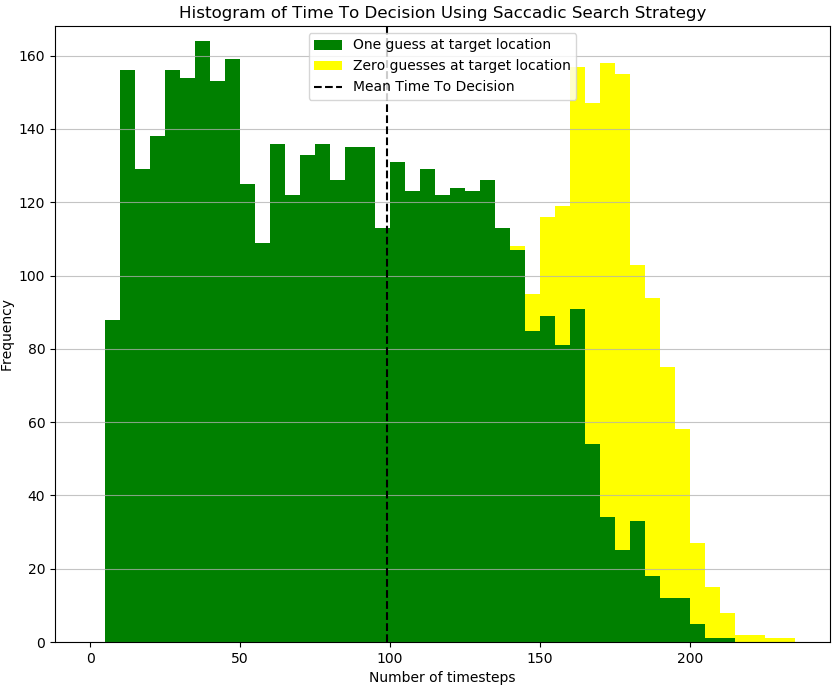
\includegraphics[width=49mm, height=49mm]{Chapters/MultiAgentTargetDetection/Figs/Histograms/VaryingPrior/Uniform/UniformSaccadicHistogram.png}
    \end{minipage}
    \\
    \hline
   
  \end{tabular}
  \caption{insert caption. }\label{table:ORToolsResults}
  %Results of running the target localisation simulation with a  uniform initial belief distribution and Gaussian initial belief distribution. p(T \Romannum{1}) = The probability of making a type \Romannum{1} error using the SPRT, p(T \Romannum{2}) = The probability of making a type \Romannum{1} error using the SPRT, Sim. FPR = The simulated false positive rate of the sensor, Sim. FNR = The simulated false negative rate of the sensor, E[TTD] = The expected amount of timesteps until a decision is made, Prec. = precision, Rec. = Recall
\end{table}

\break


\vspace*{\fill}
\section{Histograms of Time To Decision (TTD) with varying cumulative initial belief in target presence}

%Varying cumulative init belief
\begin{table}[h!]
  \centering
  \begin{tabular}{ | c | c | c | c | c |}
    \hline
    & $\epsilon$-Greedy & Sweep & Random & Saccadic \\
    \hline
    % \multicolumn{2}{c}{Initial Uniform Distribution of Belief Over Grid Cells}\\
    %\hline
    %single RAV
    %\begin{minipage}[c][height][c]{width}
    %\rotatebox[origin=c]{90}{0.75} & 
    0.75 & 
    \begin{minipage}[c][48mm][c]{48mm}
      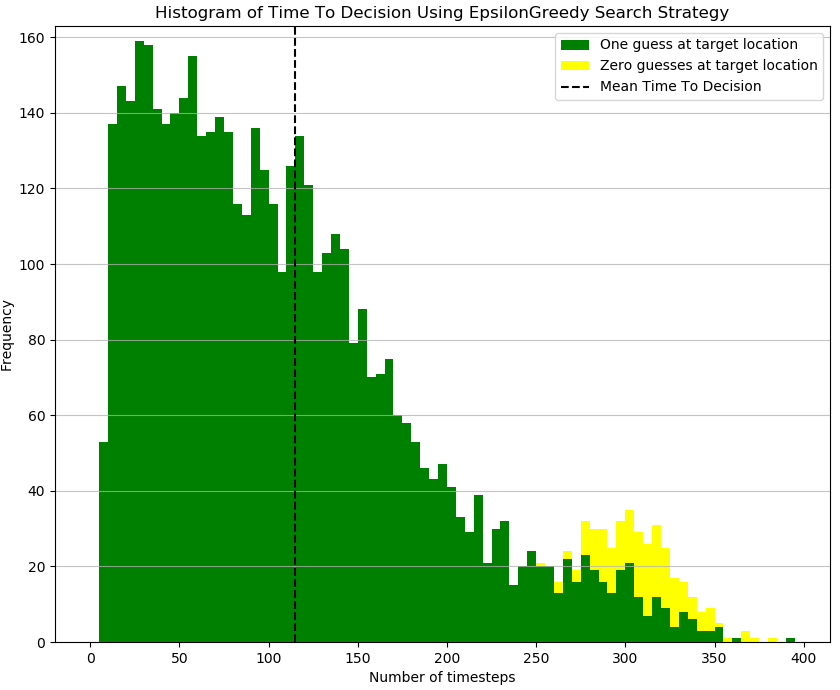
\includegraphics[width=48mm, height=48mm]{Chapters/MultiAgentTargetDetection/Figs/Histograms/VaryingInitBelief/75/75EpsilonGreedyHistogram.png}
    \end{minipage}
    &
    %\hline
    %\multicolumn{2}{c}{Initial Discretised Gaussian Distribution of Belief Over Grid Cells (random mean, covariance matrix = [[], []]}\\
    %\hline
    %single RAV
    %\begin{minipage}[c][height][c]{width}
    \begin{minipage}[c][48mm][c]{48mm}
      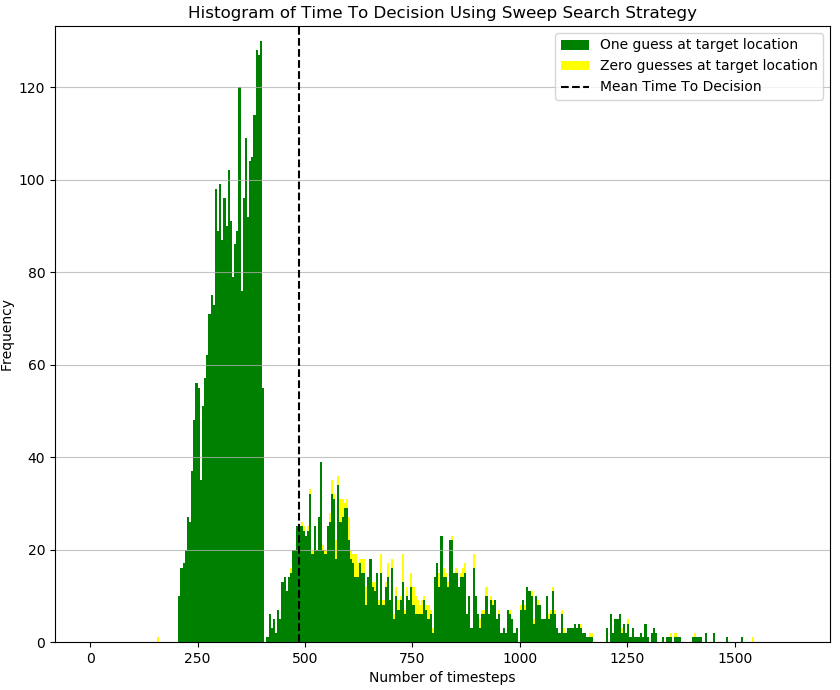
\includegraphics[width=48mm, height=48mm]{Chapters/MultiAgentTargetDetection/Figs/Histograms/VaryingInitBelief/75/75SweepHistogram.png}

    \end{minipage}
    &
    \begin{minipage}[c][48mm][c]{48mm}
      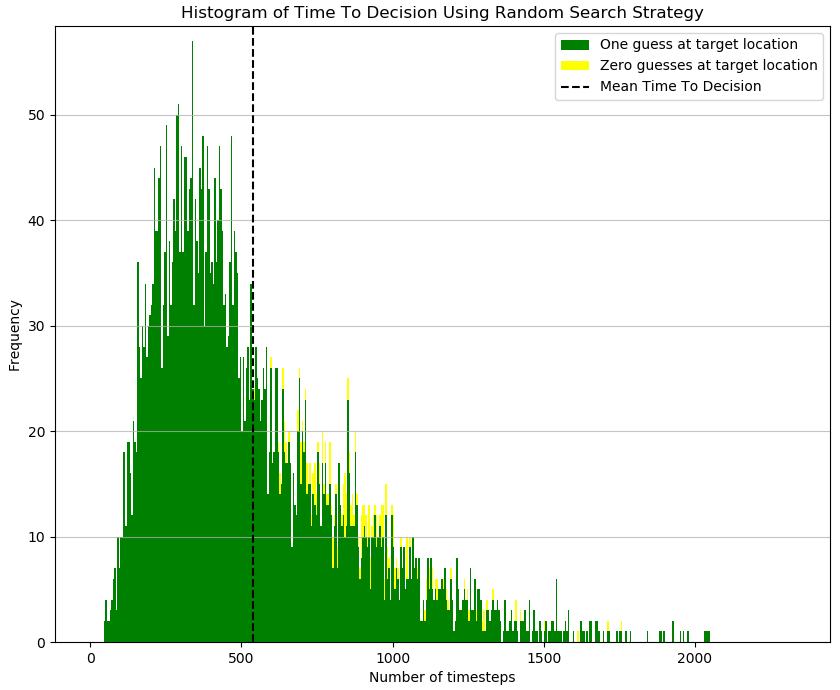
\includegraphics[width=48mm, height=48mm]{Chapters/MultiAgentTargetDetection/Figs/Histograms/VaryingInitBelief/75/75RandomHistogram.png}
    \end{minipage}
    &
    \begin{minipage}[c][48mm][c]{48mm}
      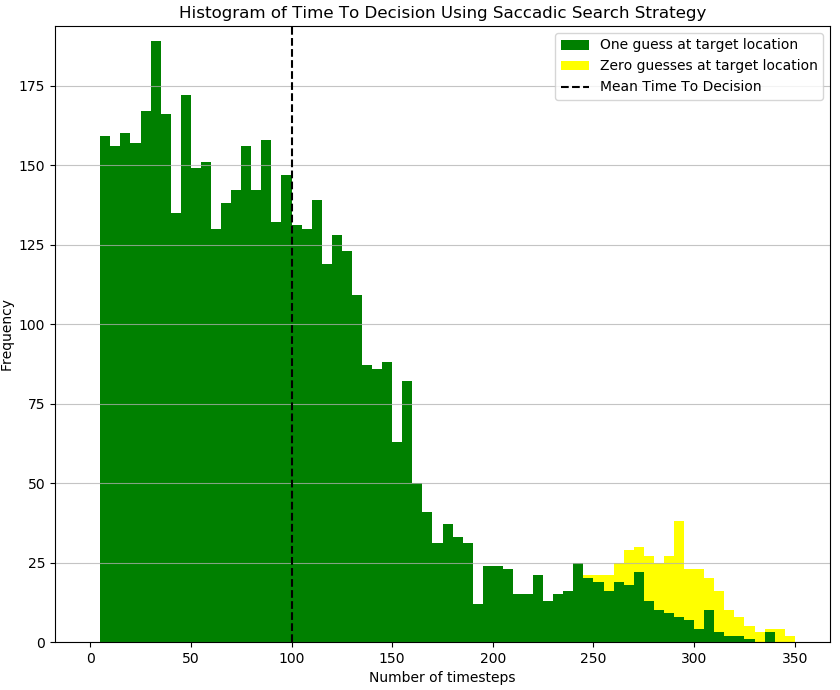
\includegraphics[width=48mm, height=48mm]{Chapters/MultiAgentTargetDetection/Figs/Histograms/VaryingInitBelief/75/75SaccadicHistogram.png}
    \end{minipage}
    \\
    %&
    %\small
    %\begin{tabular}{c|c|c|c|c|c|c|c}
    %    Strategy & p(T \Romannum{1}) & p(T \Romannum{2}) & Sim. FPR & Sim. FNR & E[TTD] & Prec. & Rec \\
    %    \hline
    %    $\epsilon$ -Greedy& 4 & 2 & 0.05 & 233.2 & 2303.3 & 2 & 9\\
    %    Sweep & 4 & 2 & 0.05 & 233.2 & 2303.3 & 2 & 9\\
    %    Saccadic & 4 & 2 & 0.05 & 233.2 & 2303.3 & 2 & 9\\
    %    Random & 4 & 2 & 0.05 & 233.2 & 2303.3 & 2 & 9\\

    %\end{tabular}
    %\normalsize
    %\rotatebox[origin=c]{90}{0.25} & 
    0.25 &
    \begin{minipage}[c][48mm][c]{48mm}
      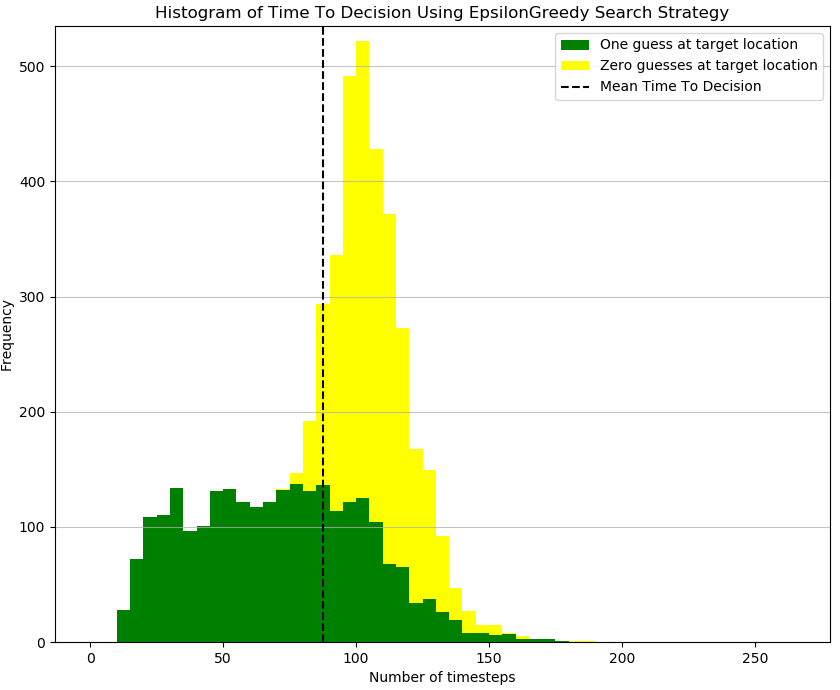
\includegraphics[width=48mm, height=48mm]{Chapters/MultiAgentTargetDetection/Figs/Histograms/VaryingInitBelief/25/25EpsilonGreedyHistogram.png}
    \end{minipage}
    &
    %\hline
    %\multicolumn{2}{c}{Initial Discretised Gaussian Distribution of Belief Over Grid Cells (random mean, covariance matrix = [[], []]}\\
    %\hline
    %single RAV
    %\begin{minipage}[c][height][c]{width}
    \begin{minipage}[c][48mm][c]{48mm}
      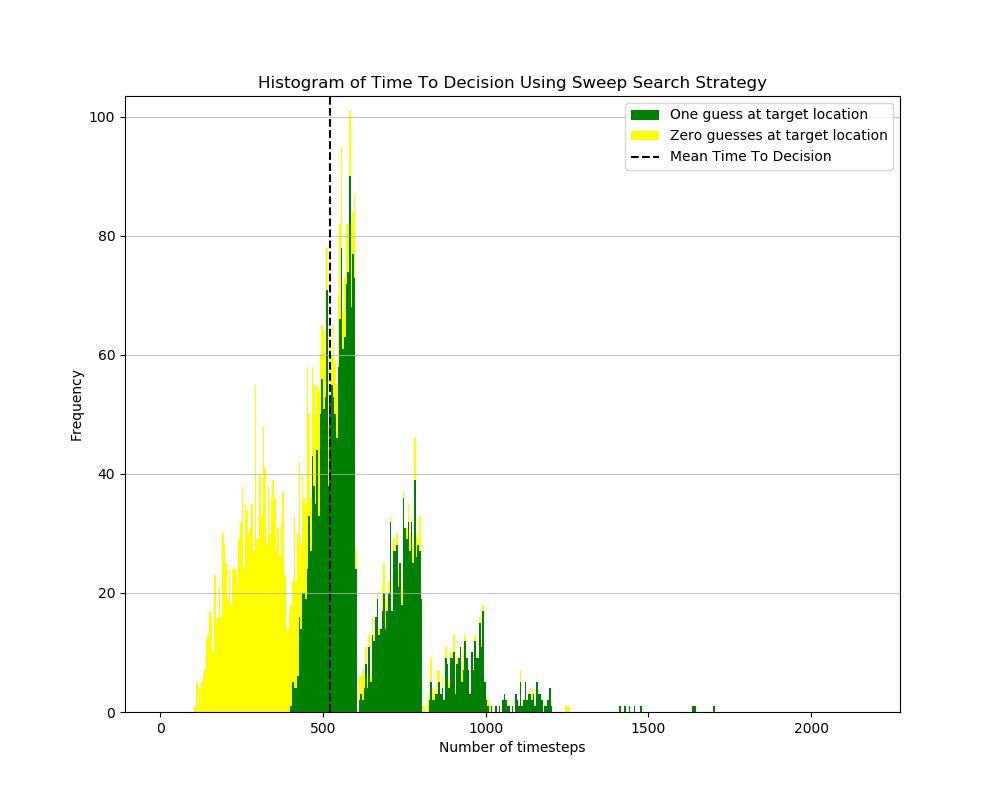
\includegraphics[width=48mm, height=48mm]{Chapters/MultiAgentTargetDetection/Figs/Histograms/VaryingInitBelief/25/25SweepHistogram.png}

    \end{minipage}
    &
    \begin{minipage}[c][48mm][c]{48mm}
      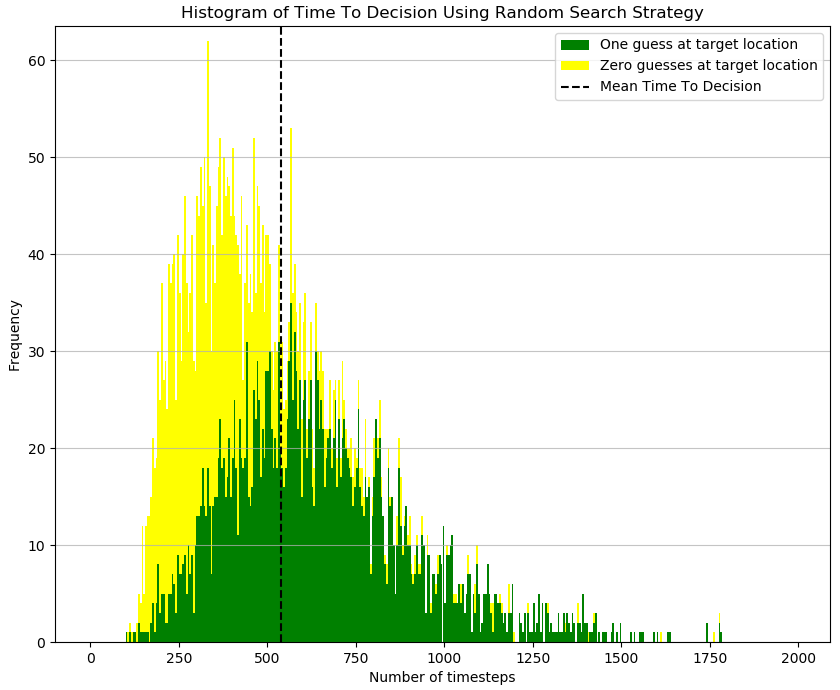
\includegraphics[width=48mm, height=48mm]{Chapters/MultiAgentTargetDetection/Figs/Histograms/VaryingInitBelief/25/25RandomHistogram.png}
    \end{minipage}
    &
    \begin{minipage}[c][48mm][c]{48mm}
      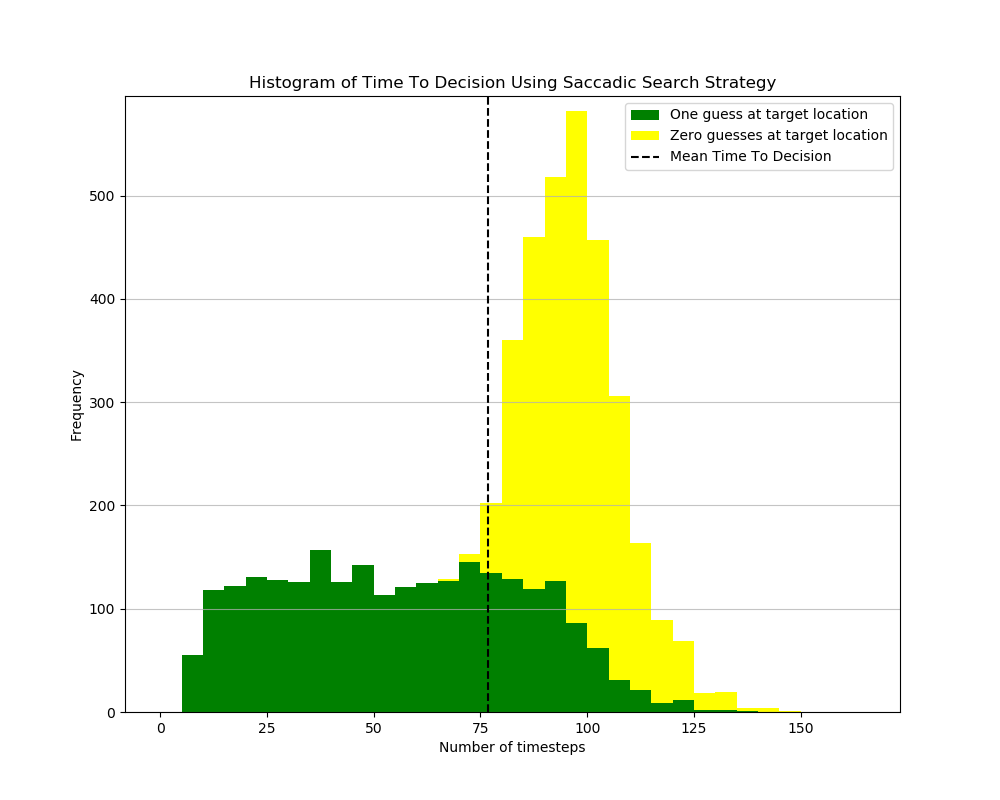
\includegraphics[width=48mm, height=48mm]{Chapters/MultiAgentTargetDetection/Figs/Histograms/VaryingInitBelief/25/25SaccadicHistogram.png}
    \end{minipage}
    \\
    \hline
   
  \end{tabular}
  \caption{insert caption. }\label{table:ORToolsResults}
\end{table}
\break




\vspace*{\fill}
\section{Histograms of Time To Decision (TTD) with varying sensor model params}

%Varying miscalibrated sensor params
\begin{table}[h!]
  \centering
  \begin{tabular}{ | m{8mm} | c | c | c | c |}
    \hline
    & $\epsilon$-Greedy & Sweep & Random & Saccadic \\
    \hline
    % \multicolumn{2}{c}{Initial Uniform Distribution of Belief Over Grid Cells}\\
    %\hline
    %single RAV
    %\begin{minipage}[c][height][c]{width}
    %\rotatebox[origin=c]{90}{0.4/0.4} & 
    0.4/ 0.4 &
    \begin{minipage}[c][48mm][c]{48mm}
      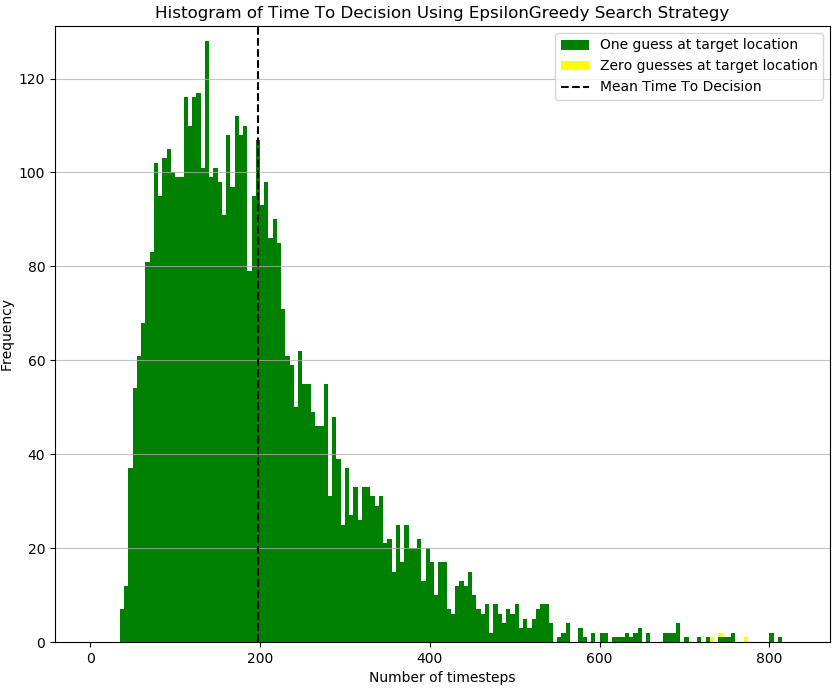
\includegraphics[width=48mm, height=48mm]{Chapters/MultiAgentTargetDetection/Figs/Histograms/MiscalibratedSensor/4-4/4-4EpsilonGreedyHistogram.png}
    \end{minipage}
    &
    %\hline
    %\multicolumn{2}{c}{Initial Discretised Gaussian Distribution of Belief Over Grid Cells (random mean, covariance matrix = [[], []]}\\
    %\hline
    %single RAV
    %\begin{minipage}[c][height][c]{width}
    \begin{minipage}[c][48mm][c]{48mm}
      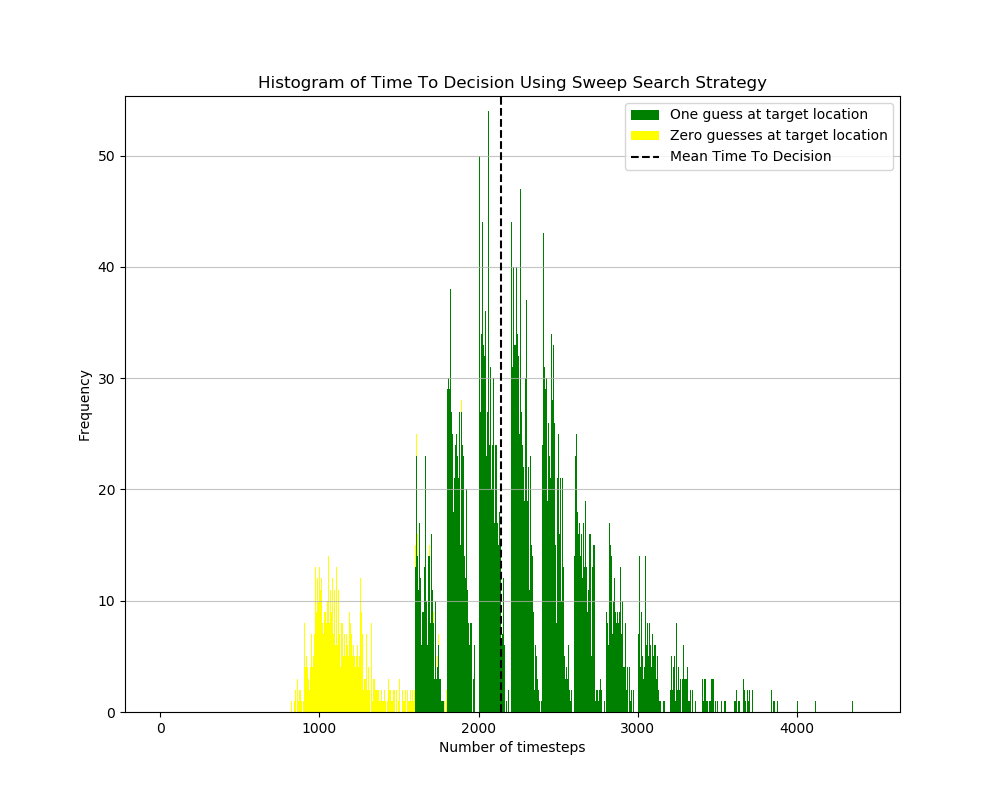
\includegraphics[width=48mm, height=48mm]{Chapters/MultiAgentTargetDetection/Figs/Histograms/MiscalibratedSensor/4-4/4-4SweepHistogram.png}

    \end{minipage}
    &
    \begin{minipage}[c][48mm][c]{48mm}
      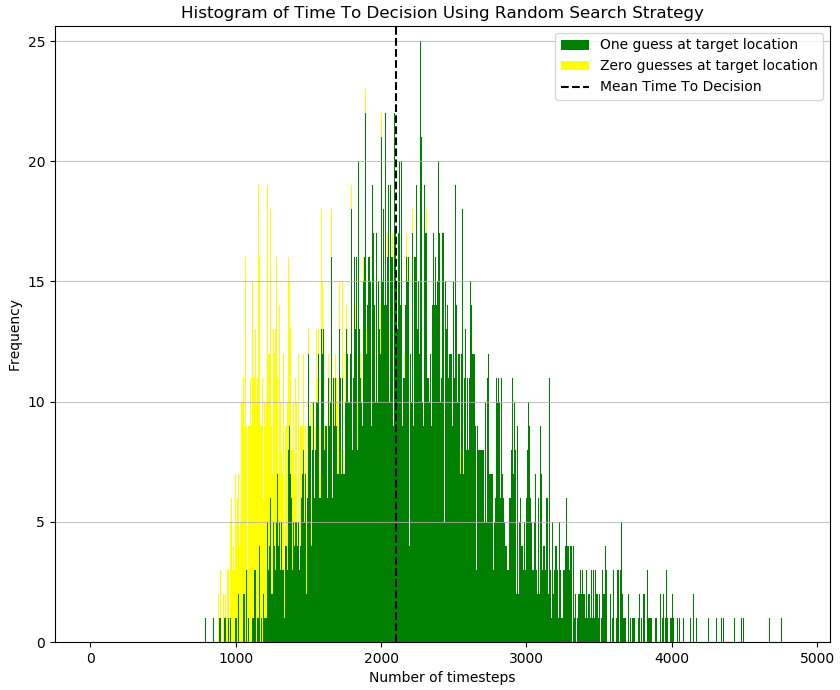
\includegraphics[width=48mm, height=48mm]{Chapters/MultiAgentTargetDetection/Figs/Histograms/MiscalibratedSensor/4-4/4-4RandomHistogram.png}
    \end{minipage}
    &
    \begin{minipage}[c][48mm][c]{48mm}
      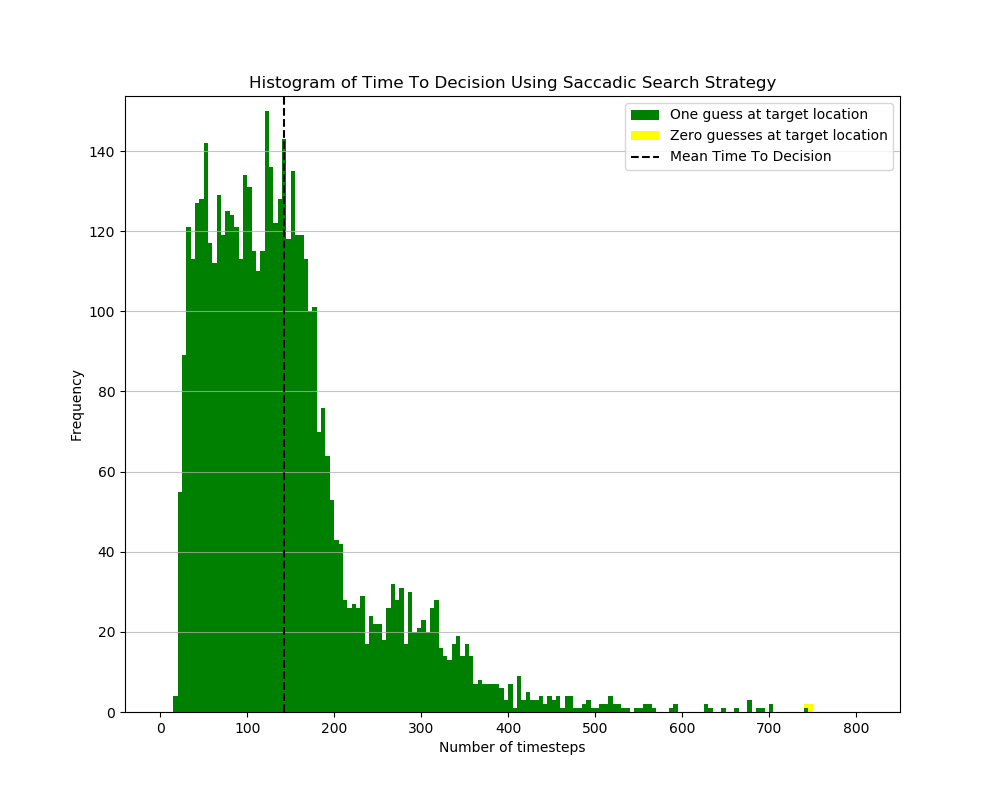
\includegraphics[width=48mm, height=48mm]{Chapters/MultiAgentTargetDetection/Figs/Histograms/MiscalibratedSensor/4-4/4-4SaccadicHistogram.png}
    \end{minipage}
    \\
    %&
    %\small
    %\begin{tabular}{c|c|c|c|c|c|c|c}
    %    Strategy & p(T \Romannum{1}) & p(T \Romannum{2}) & Sim. FPR & Sim. FNR & E[TTD] & Prec. & Rec \\
    %    \hline
    %    $\epsilon$ -Greedy& 4 & 2 & 0.05 & 233.2 & 2303.3 & 2 & 9\\
    %    Sweep & 4 & 2 & 0.05 & 233.2 & 2303.3 & 2 & 9\\
    %    Saccadic & 4 & 2 & 0.05 & 233.2 & 2303.3 & 2 & 9\\
    %    Random & 4 & 2 & 0.05 & 233.2 & 2303.3 & 2 & 9\\

    %\end{tabular}
    %\normalsize
    %\rotatebox[origin=c]{90}{0.05.0.02} & \vline
    0.05/ 0.02 &
    \begin{minipage}[c][48mm][c]{48mm}
      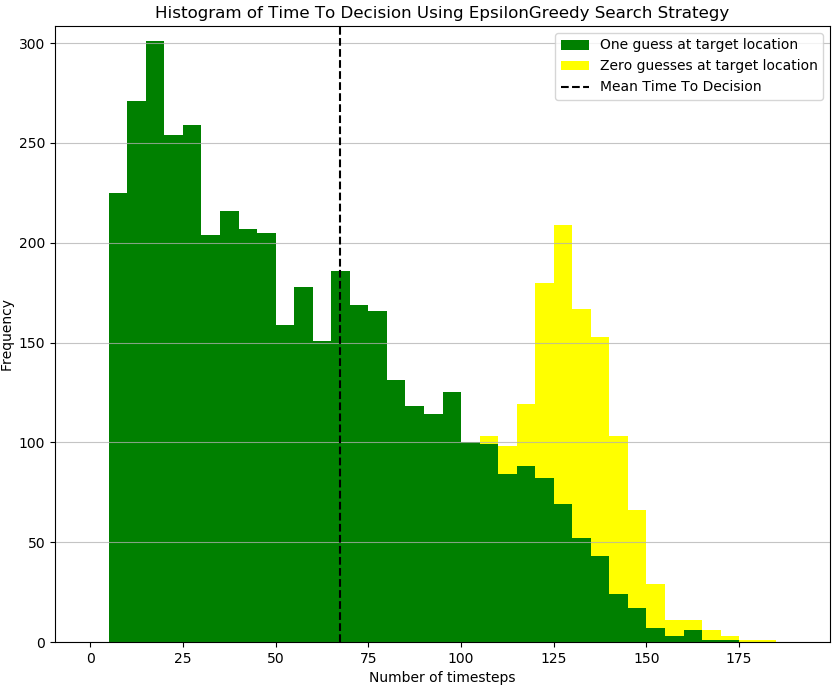
\includegraphics[width=48mm, height=48mm]{Chapters/MultiAgentTargetDetection/Figs/Histograms/MiscalibratedSensor/05-02/05-02EpsilonGreedyHistogram.png}
    \end{minipage}
    &
    %\hline
    %\multicolumn{2}{c}{Initial Discretised Gaussian Distribution of Belief Over Grid Cells (random mean, covariance matrix = [[], []]}\\
    %\hline
    %single RAV
    %\begin{minipage}[c][height][c]{width}
    \begin{minipage}[c][48mm][c]{48mm}
      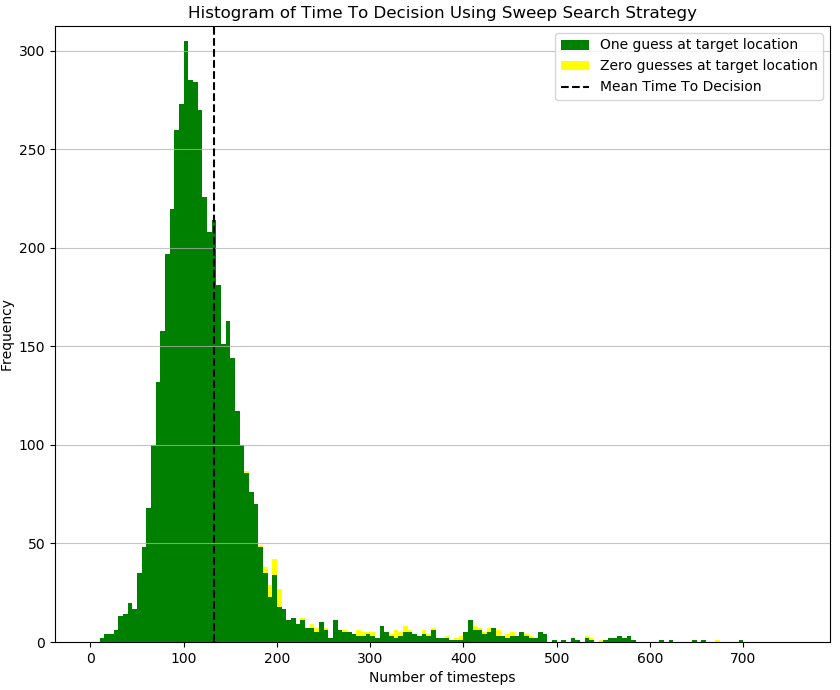
\includegraphics[width=48mm, height=48mm]{Chapters/MultiAgentTargetDetection/Figs/Histograms/MiscalibratedSensor/05-02/05-02SweepHistogram.png}

    \end{minipage}
    &
    \begin{minipage}[c][48mm][c]{48mm}
      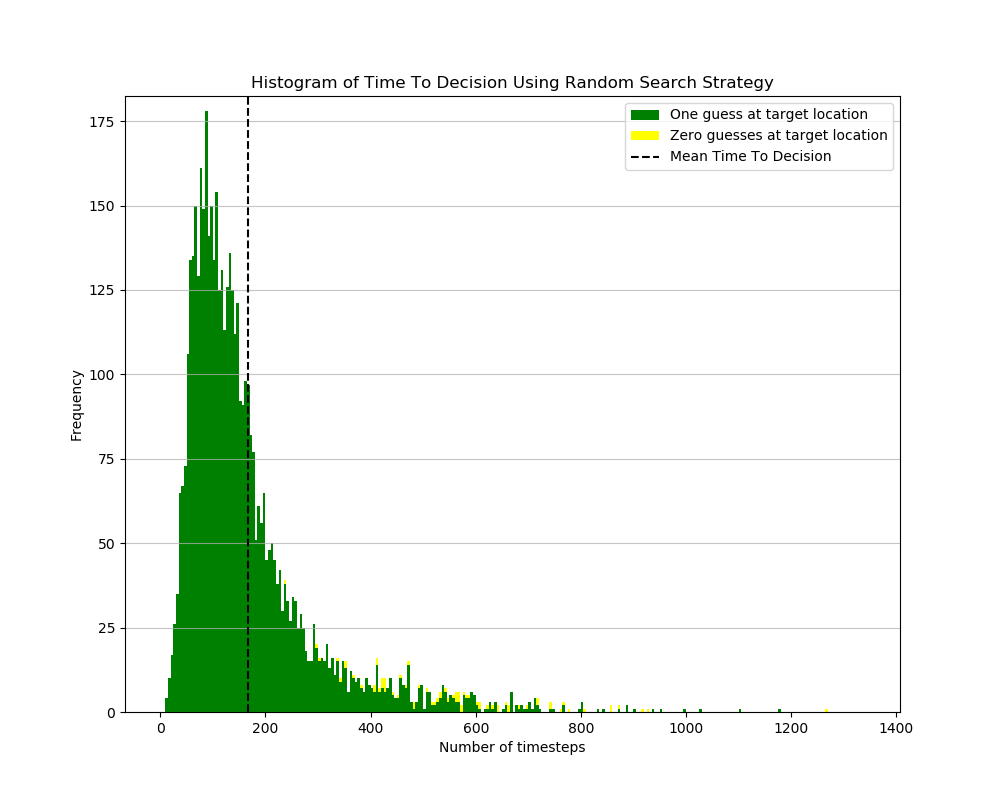
\includegraphics[width=48mm, height=48mm]{Chapters/MultiAgentTargetDetection/Figs/Histograms/MiscalibratedSensor/05-02/05-02RandomHistogram.png}
    \end{minipage}
    &
    \begin{minipage}[c][48mm][c]{48mm}
      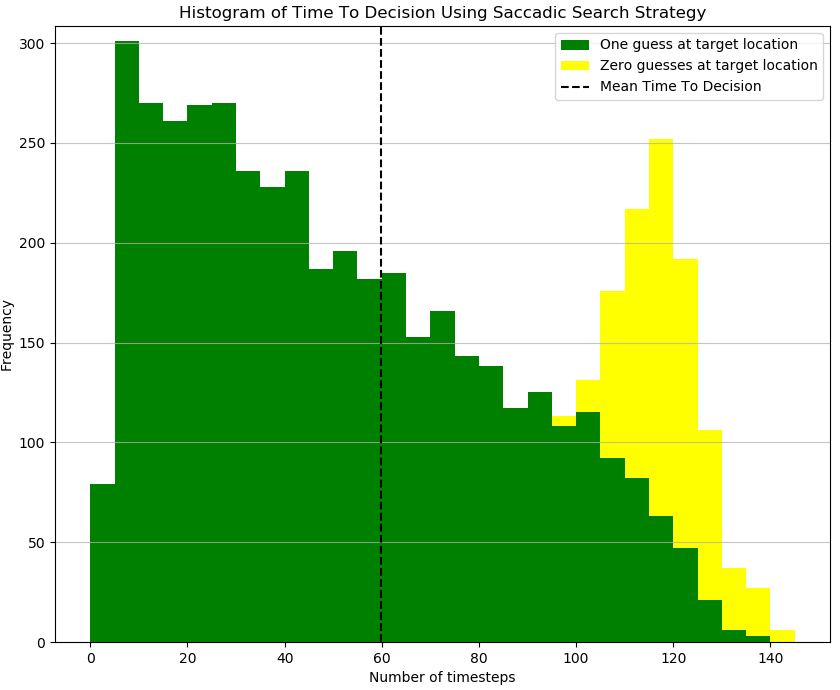
\includegraphics[width=48mm, height=48mm]{Chapters/MultiAgentTargetDetection/Figs/Histograms/MiscalibratedSensor/05-02/05-02SaccadicHistogram.png}
    \end{minipage}
    \\
    \hline
   
  \end{tabular}
  \caption{insert caption. }\label{table:ORToolsResults}
\end{table}
\break



\vspace*{\fill}
\section{Histograms of Time To Decision (TTD) with varying number of targets present}

%Varying number targets
\begin{table}[h!]
  \centering
  \begin{tabular}{ | c | c | c | c | c |}
    \hline
    & $\epsilon$-Greedy & Sweep & Random & Saccadic \\
    \hline
    % \multicolumn{2}{c}{Initial Uniform Distribution of Belief Over Grid Cells}\\
    %\hline
    %single RAV
    %\begin{minipage}[c][height][c]{width}
    2 & 
    \begin{minipage}[c][49mm][c]{49mm}
      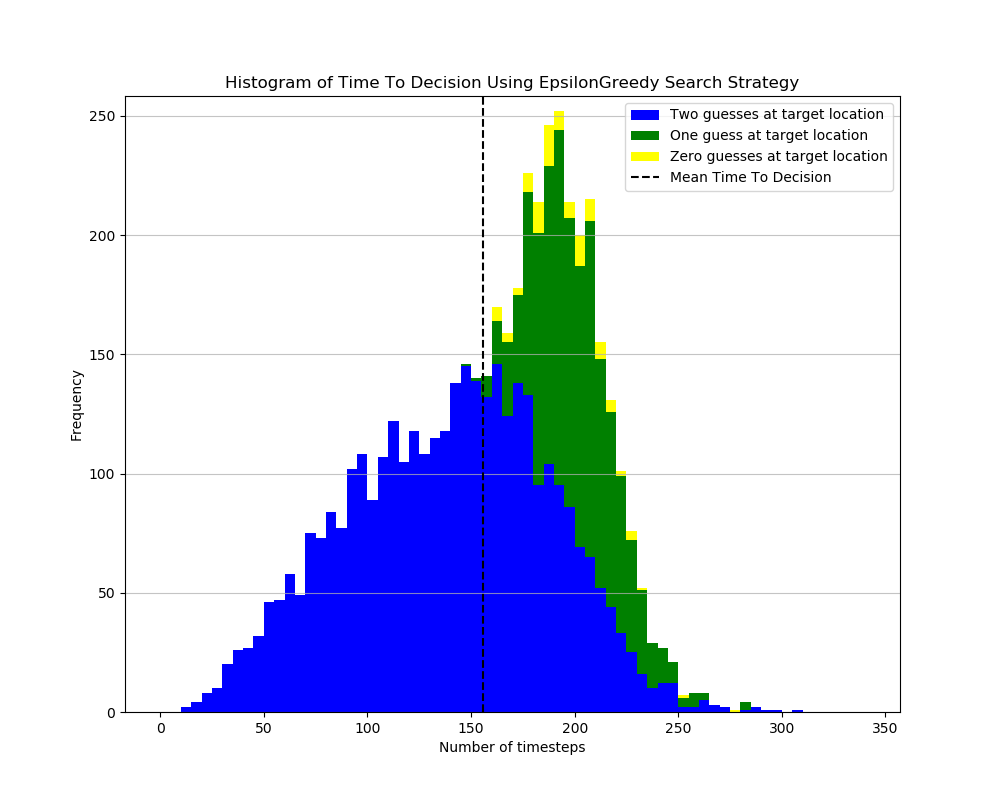
\includegraphics[width=49mm, height=49mm]{Chapters/MultiAgentTargetDetection/Figs/Histograms/MultipleTarget/2/2EpsilonGreedyHistogram.png}
    \end{minipage}
    &
    %\hline
    %\multicolumn{2}{c}{Initial Discretised Gaussian Distribution of Belief Over Grid Cells (random mean, covariance matrix = [[], []]}\\
    %\hline
    %single RAV
    %\begin{minipage}[c][height][c]{width}
    \begin{minipage}[c][49mm][c]{49mm}
      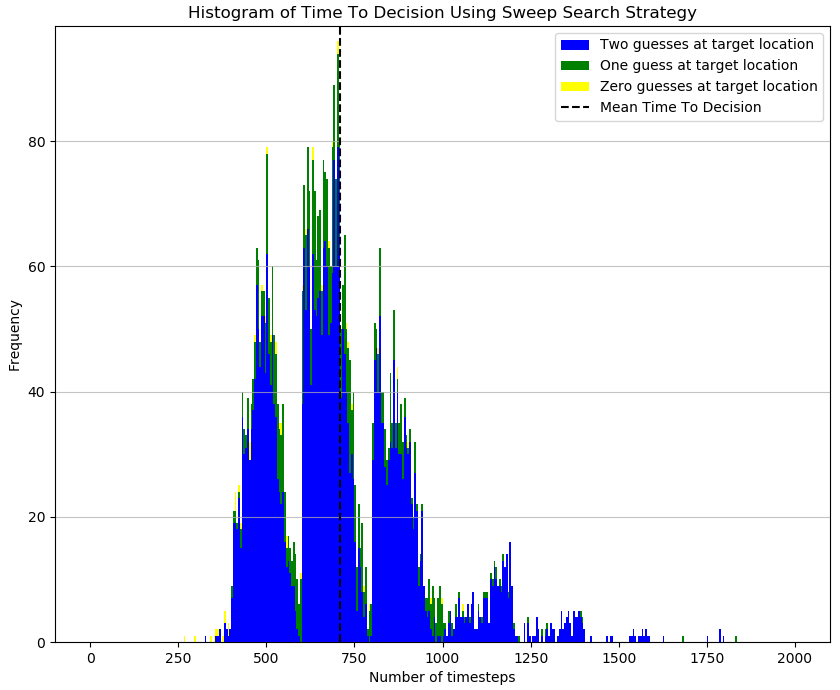
\includegraphics[width=49mm, height=49mm]{Chapters/MultiAgentTargetDetection/Figs/Histograms/MultipleTarget/2/2SweepHistogram.png}

    \end{minipage}
    &
    \begin{minipage}[c][49mm][c]{49mm}
      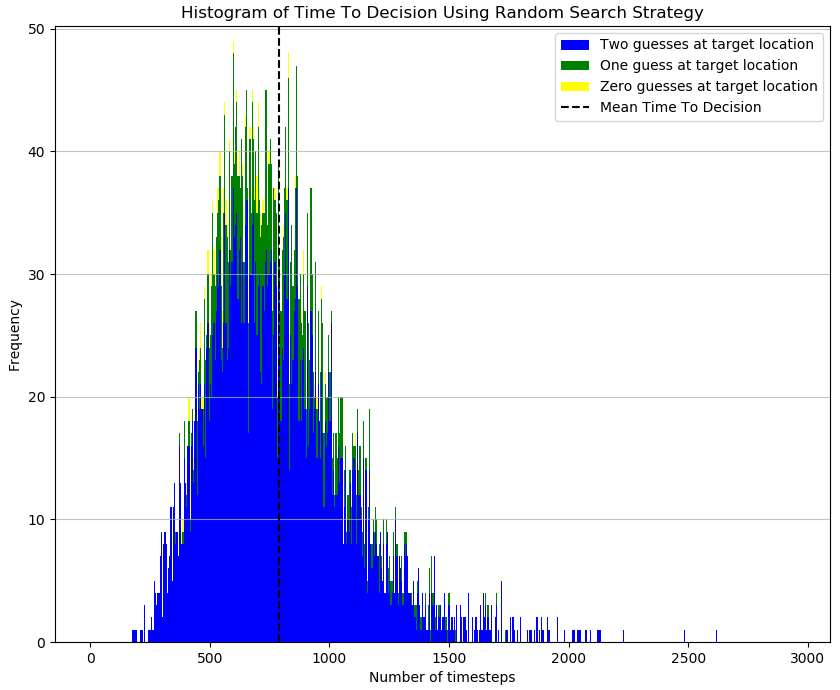
\includegraphics[width=49mm, height=49mm]{Chapters/MultiAgentTargetDetection/Figs/Histograms/MultipleTarget/2/2RandomHistogram.png}
    \end{minipage}
    &
    \begin{minipage}[c][49mm][c]{49mm}
      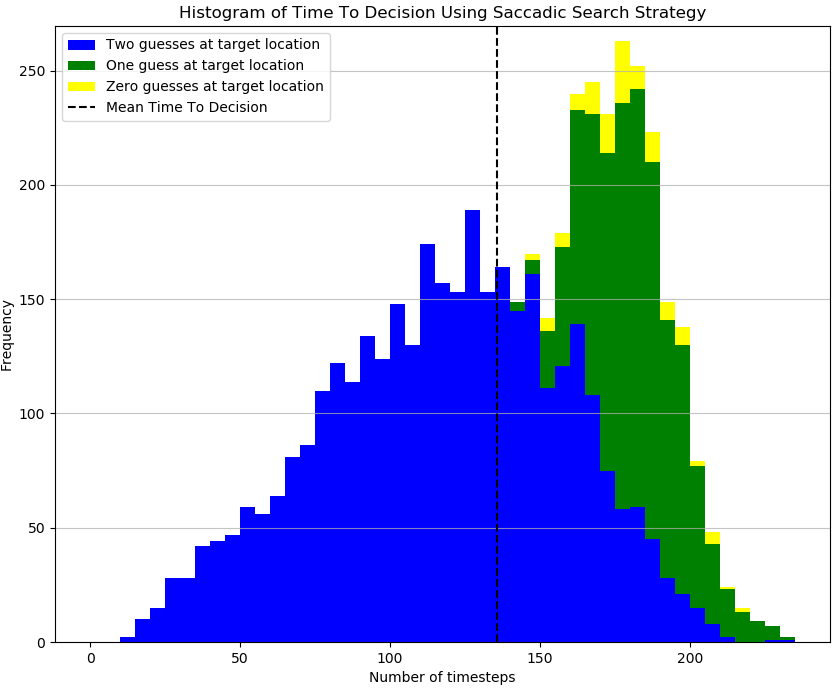
\includegraphics[width=49mm, height=49mm]{Chapters/MultiAgentTargetDetection/Figs/Histograms/MultipleTarget/2/2SaccadicHistogram.png}
    \end{minipage}
    \\
    %&
    %\small
    %\begin{tabular}{c|c|c|c|c|c|c|c}
    %    Strategy & p(T \Romannum{1}) & p(T \Romannum{2}) & Sim. FPR & Sim. FNR & E[TTD] & Prec. & Rec \\
    %    \hline
    %    $\epsilon$ -Greedy& 4 & 2 & 0.05 & 233.2 & 2303.3 & 2 & 9\\
    %    Sweep & 4 & 2 & 0.05 & 233.2 & 2303.3 & 2 & 9\\
    %    Saccadic & 4 & 2 & 0.05 & 233.2 & 2303.3 & 2 & 9\\
    %    Random & 4 & 2 & 0.05 & 233.2 & 2303.3 & 2 & 9\\

    %\end{tabular}
    %\normalsize
    3 & 
    \begin{minipage}[c][49mm][c]{49mm}
      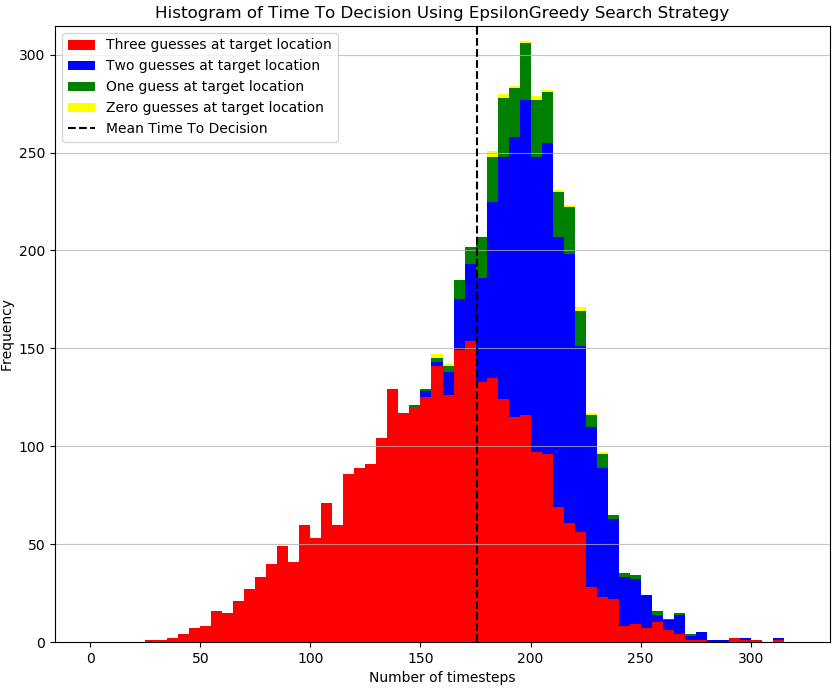
\includegraphics[width=49mm, height=49mm]{Chapters/MultiAgentTargetDetection/Figs/Histograms/MultipleTarget/3/3EpsilonGreedyHistogram.png}
    \end{minipage}
    &
    %\hline
    %\multicolumn{2}{c}{Initial Discretised Gaussian Distribution of Belief Over Grid Cells (random mean, covariance matrix = [[], []]}\\
    %\hline
    %single RAV
    %\begin{minipage}[c][height][c]{width}
    \begin{minipage}[c][49mm][c]{49mm}
      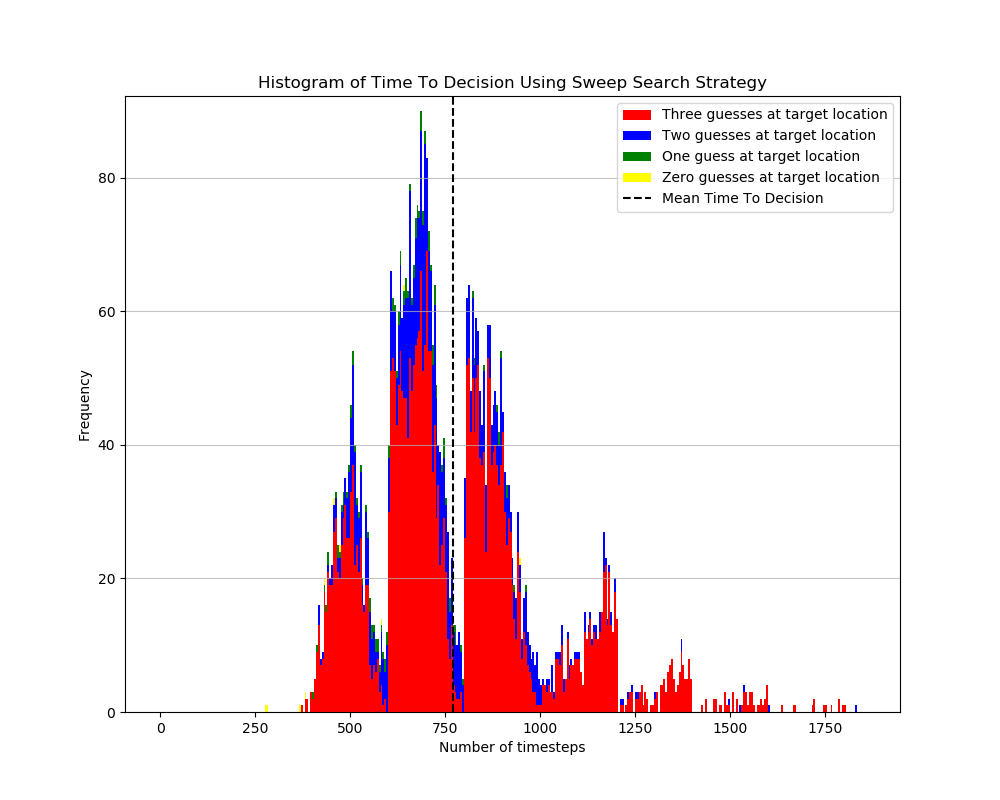
\includegraphics[width=49mm, height=49mm]{Chapters/MultiAgentTargetDetection/Figs/Histograms/MultipleTarget/3/3SweepHistogram.png}

    \end{minipage}
    &
    \begin{minipage}[c][49mm][c]{49mm}
      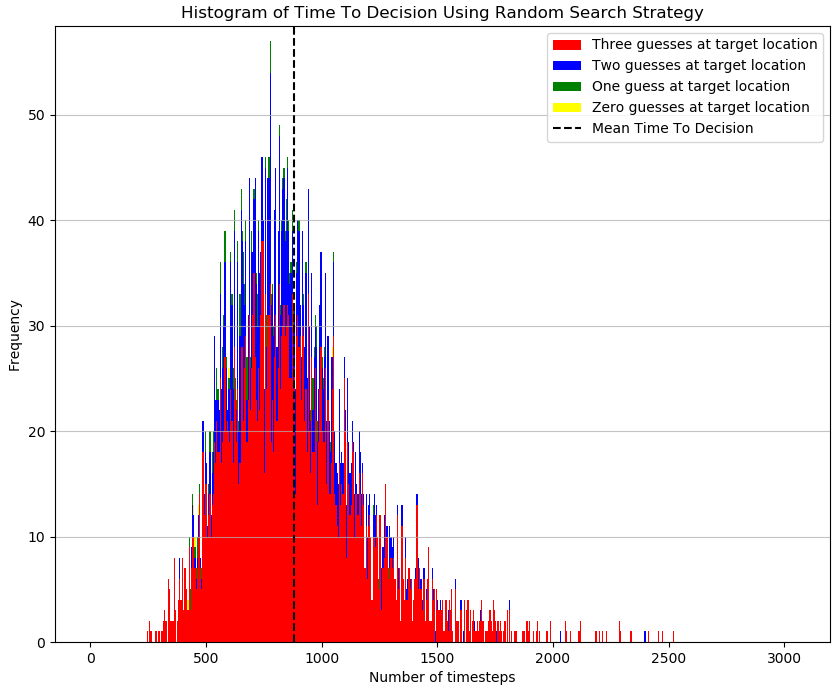
\includegraphics[width=49mm, height=49mm]{Chapters/MultiAgentTargetDetection/Figs/Histograms/MultipleTarget/3/3RandomHistogram.png}
    \end{minipage}
    &
    \begin{minipage}[c][49mm][c]{49mm}
      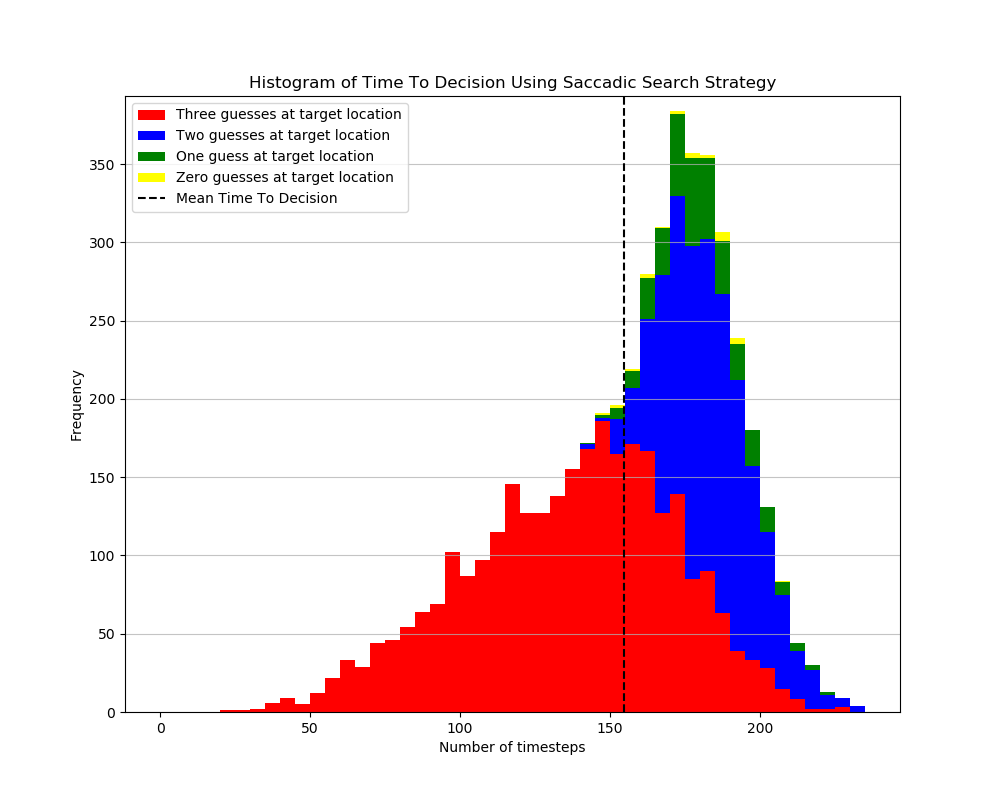
\includegraphics[width=49mm, height=49mm]{Chapters/MultiAgentTargetDetection/Figs/Histograms/MultipleTarget/3/3SaccadicHistogram.png}
    \end{minipage}
    \\
    \hline
   
  \end{tabular}
  \caption{insert caption. }\label{table:ORToolsResults}
\end{table}
\break




\vspace*{\fill}
\section{Histograms of Time To Decision (TTD) with varying number of search agents}

%Varying number agents
\begin{table}[h!]
  \centering
  \begin{tabular}{ | c | c | c | c | c |}
    \hline
    & $\epsilon$-Greedy & Sweep & Random & Saccadic \\
    \hline
    % \multicolumn{2}{c}{Initial Uniform Distribution of Belief Over Grid Cells}\\
    %\hline
    %single RAV
    %\begin{minipage}[c][height][c]{width}
    2 & 
    \begin{minipage}[c][49mm][c]{49mm}
      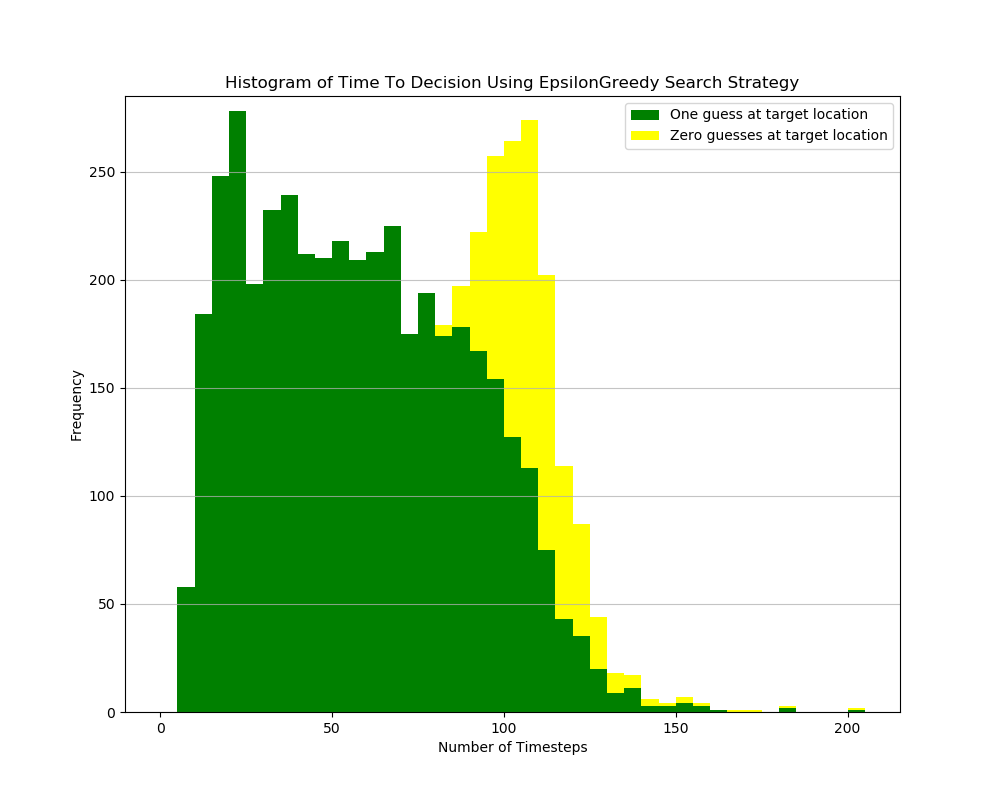
\includegraphics[width=49mm, height=49mm]{Chapters/MultiAgentTargetDetection/Figs/Histograms/MultipleAgent/2/SingleAgentSingleSource2EpsilonGreedyHistogram.png}
    \end{minipage}
    &
    %\hline
    %\multicolumn{2}{c}{Initial Discretised Gaussian Distribution of Belief Over Grid Cells (random mean, covariance matrix = [[], []]}\\
    %\hline
    %single RAV
    %\begin{minipage}[c][height][c]{width}
    \begin{minipage}[c][49mm][c]{49mm}
      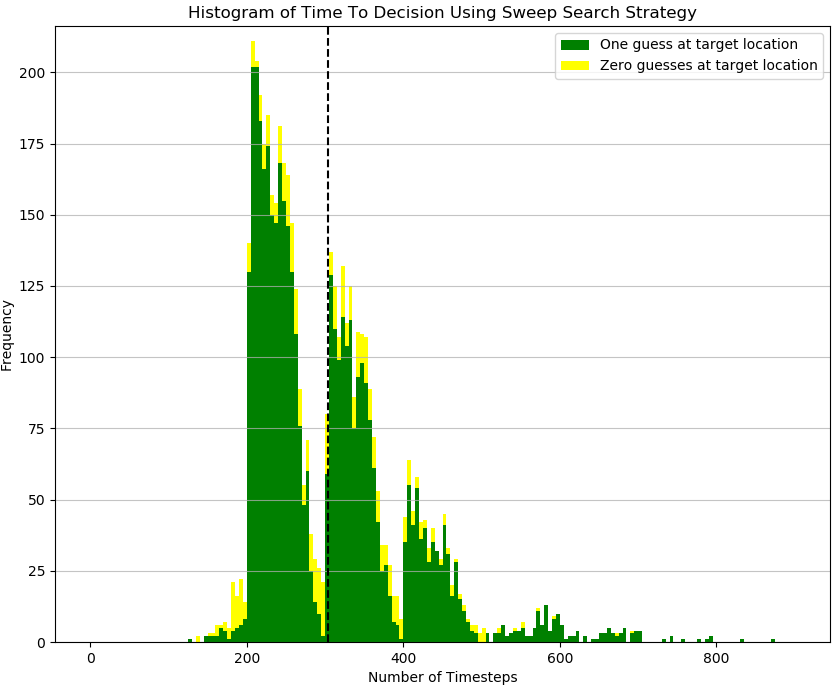
\includegraphics[width=49mm, height=49mm]{Chapters/MultiAgentTargetDetection/Figs/Histograms/MultipleAgent/2/SingleAgentSingleSource2SweepHistogram.png}

    \end{minipage}
    &
    \begin{minipage}[c][49mm][c]{49mm}
      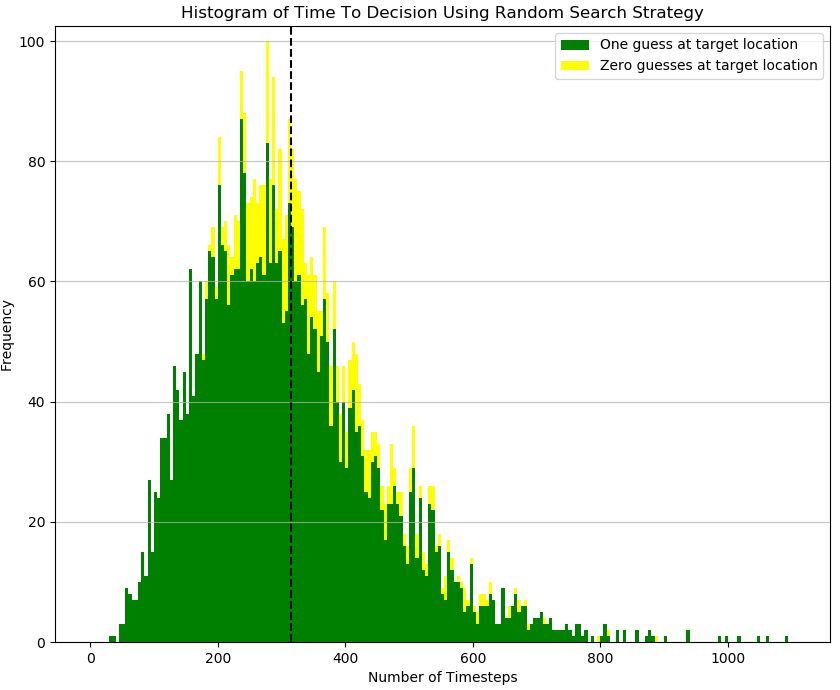
\includegraphics[width=49mm, height=49mm]{Chapters/MultiAgentTargetDetection/Figs/Histograms/MultipleAgent/2/SingleAgentSingleSource2RandomHistogram.png}
    \end{minipage}
    &
    \begin{minipage}[c][49mm][c]{49mm}
      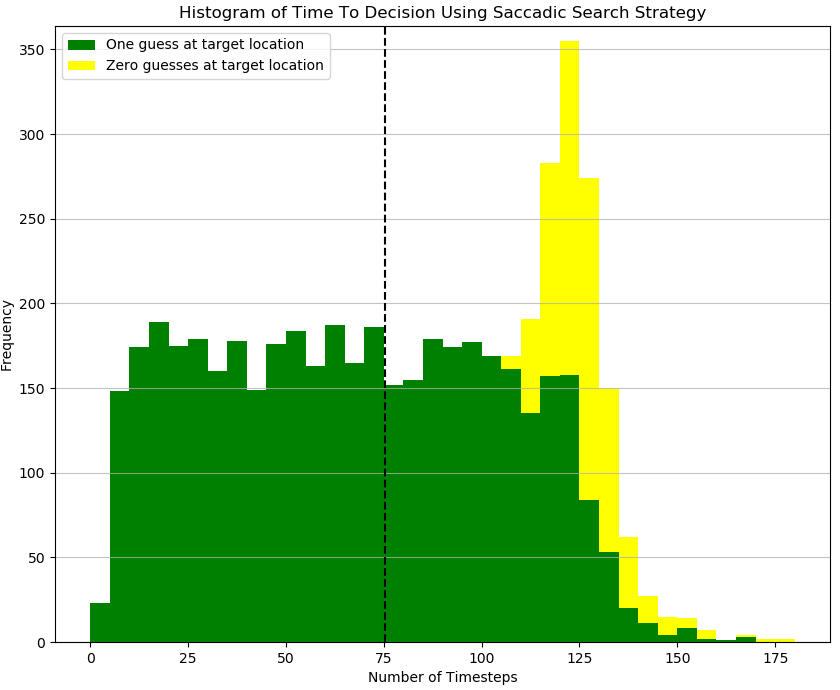
\includegraphics[width=49mm, height=49mm]{Chapters/MultiAgentTargetDetection/Figs/Histograms/MultipleAgent/2/SingleAgentSingleSource2SaccadicHistogram.png}
    \end{minipage}
    \\
    %&
    %\small
    %\begin{tabular}{c|c|c|c|c|c|c|c}
    %    Strategy & p(T \Romannum{1}) & p(T \Romannum{2}) & Sim. FPR & Sim. FNR & E[TTD] & Prec. & Rec \\
    %    \hline
    %    $\epsilon$ -Greedy& 4 & 2 & 0.05 & 233.2 & 2303.3 & 2 & 9\\
    %    Sweep & 4 & 2 & 0.05 & 233.2 & 2303.3 & 2 & 9\\
    %    Saccadic & 4 & 2 & 0.05 & 233.2 & 2303.3 & 2 & 9\\
    %    Random & 4 & 2 & 0.05 & 233.2 & 2303.3 & 2 & 9\\

    %\end{tabular}
    %\normalsize
    3 & 
    \begin{minipage}[c][49mm][c]{49mm}
      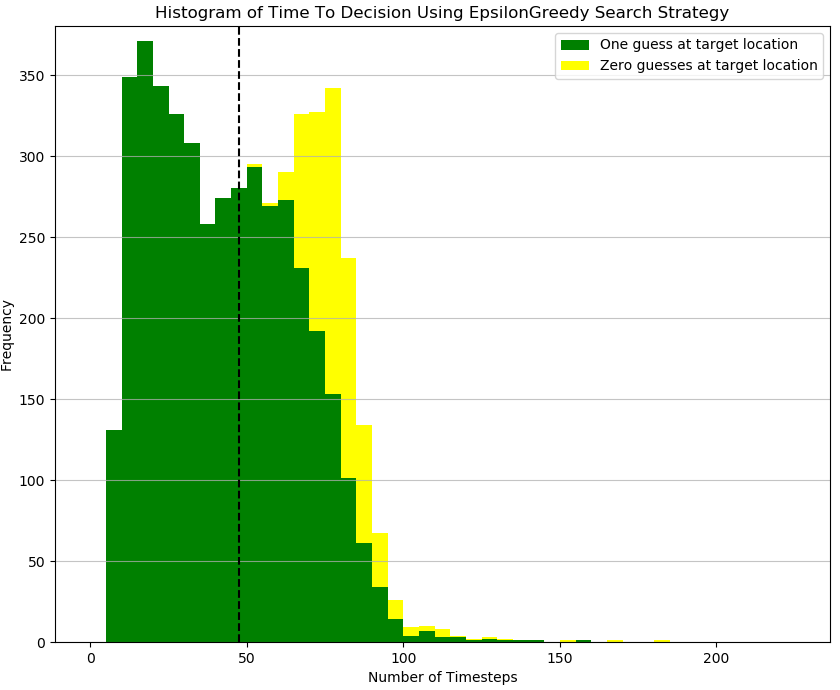
\includegraphics[width=49mm, height=49mm]{Chapters/MultiAgentTargetDetection/Figs/Histograms/MultipleAgent/3/SingleAgentSingleSource3EpsilonGreedyHistogram.png}
    \end{minipage}
    &
    %\hline
    %\multicolumn{2}{c}{Initial Discretised Gaussian Distribution of Belief Over Grid Cells (random mean, covariance matrix = [[], []]}\\
    %\hline
    %single RAV
    %\begin{minipage}[c][height][c]{width}
    \begin{minipage}[c][49mm][c]{49mm}
      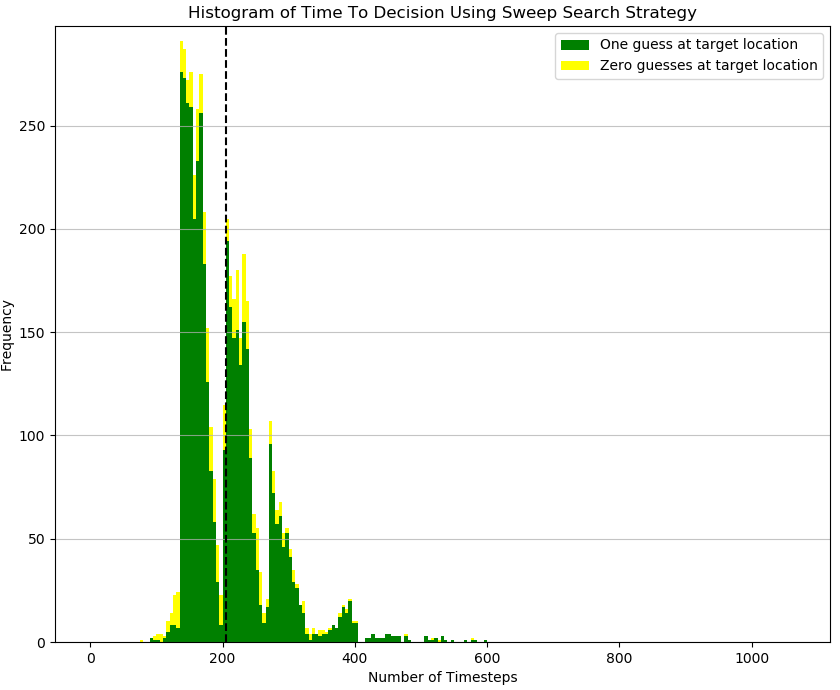
\includegraphics[width=49mm, height=49mm]{Chapters/MultiAgentTargetDetection/Figs/Histograms/MultipleAgent/3/SingleAgentSingleSource3SweepHistogram.png}

    \end{minipage}
    &
    \begin{minipage}[c][49mm][c]{49mm}
      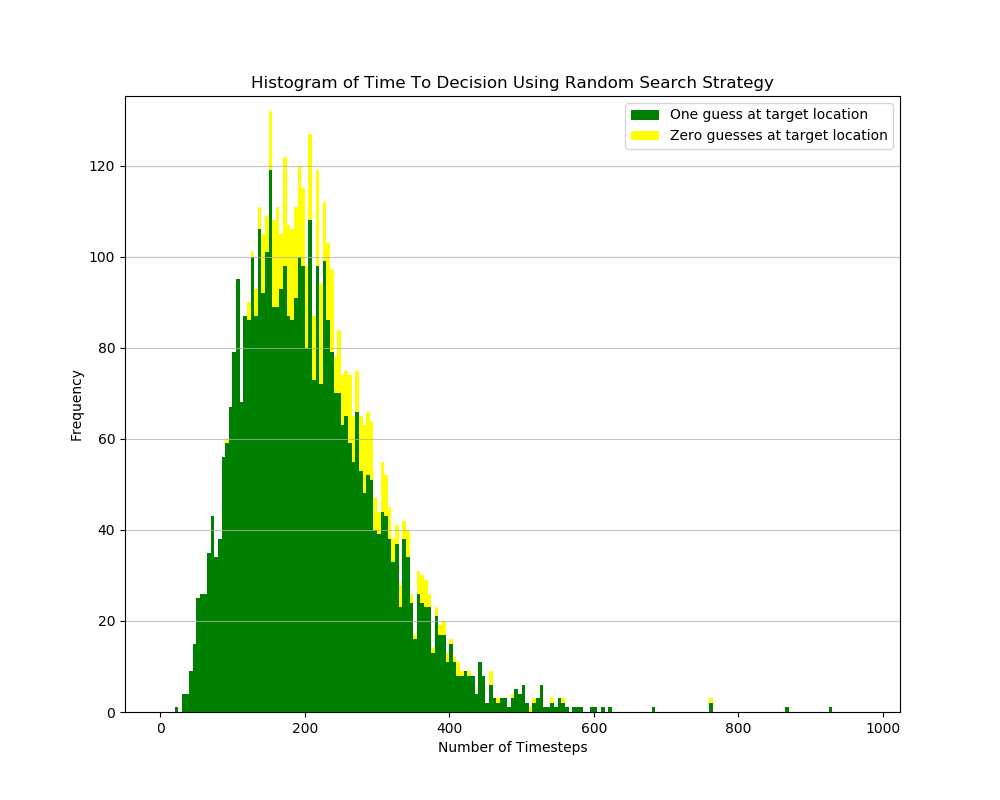
\includegraphics[width=49mm, height=49mm]{Chapters/MultiAgentTargetDetection/Figs/Histograms/MultipleAgent/3/SingleAgentSingleSource3RandomHistogram.png}
    \end{minipage}
    &
    \begin{minipage}[c][49mm][c]{49mm}
      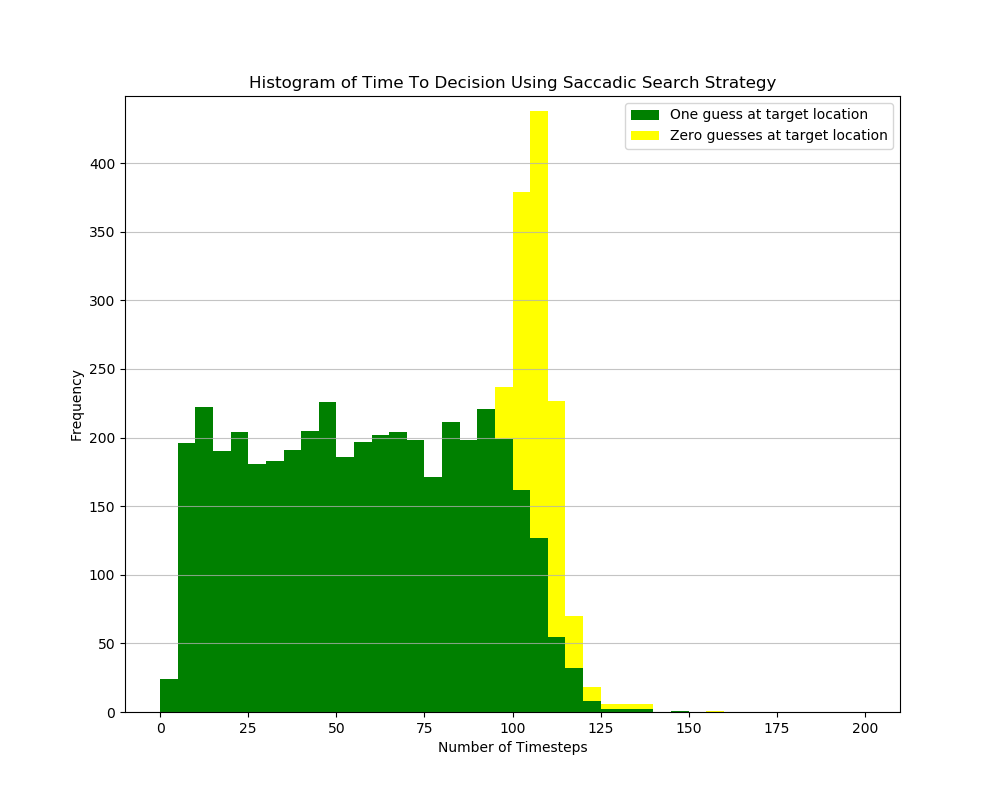
\includegraphics[width=49mm, height=49mm]{Chapters/MultiAgentTargetDetection/Figs/Histograms/MultipleAgent/3/SingleAgentSingleSource3SaccadicHistogram.png}
    \end{minipage}
    \\
    \hline
   
  \end{tabular}
  \caption{insert caption. }\label{table:ORToolsResults}
\end{table}


\end{landscape}
